\section{Analysis technique}

\begin{frame}{Stacked analysis}
\begin{minipage}[c]{0.45\textwidth}
%57
  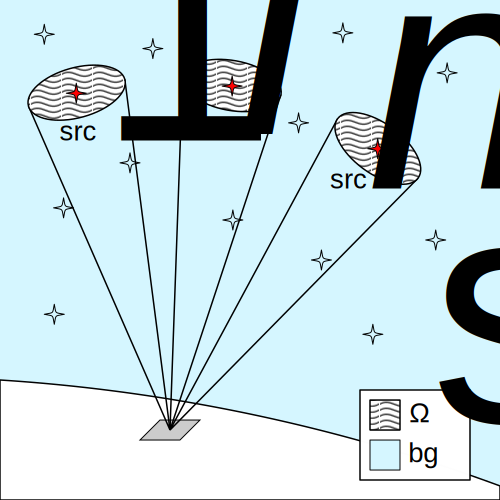
\includegraphics[width=1\textwidth]{pics/stacked.pdf}
\end{minipage}
\hfill
\begin{minipage}[c]{0.52\textwidth}
%39
{
\Large
\[
\frac{\sum_{i=1}^n N_i^\mathsf{src}}{\sum_{i=1}^n \Omega_i^\mathsf{src}} \stackrel{?}{>}
\frac{N^\mathsf{bg}}{\Omega^\mathsf{bg}}
\]
}
\small

\textcolor{kit-green100}{$N_i^\mathsf{src}$} is a number of events for \\the \textcolor{kit-green100}{$i$}-th source,\\
\textcolor{kit-green100}{$\Omega_i^\mathsf{src}$} is a solid angle of the selected area of the sky around the \textcolor{kit-green100}{$i$}-th source,\\
\textcolor{kit-green100}{$N^\mathsf{bg}$} is a number of background events,\\
\textcolor{kit-green100}{$\Omega^\mathsf{bg}$} is a solid angle of the area used for background estimation.

\end{minipage}
\end{frame}


% \section{Stacked analysis example}

% \begin{frame}{Stacked analysis example: Carpet-2 high-energy $\gamma$ search}
% % Stacked analysis example: Carpet-2 high-energy gamma rays search for IceCube point sources
%     \begin{itemize}
%         \item located at the Baksan Neutrino Observatory of INR RAS;
%     \end{itemize}
%     \vspace{-0.3em}
%     \begin{minipage}[c]{0.5\textwidth}
%         \begin{itemize}
%             \item consists of:
%             \begin{itemize}
%             \item surface array to detect the electromagnetic CR components;
%             \item underground scintillator detectors to detect the muonic component;
%             \end{itemize}
%             \item used for study air showers induced by particles with primary energy above 50 TeV.
%             \item the main area $\approx 200$~m$^2$.
%         \end{itemize}
%     \end{minipage}
%     \hfill
%     \begin{minipage}[c]{0.49\textwidth}
%         \includegraphics[width=1\textwidth]{pics/CarpetLayout.pdf}
%     \end{minipage}
% \end{frame}

\begin{frame}{Example: recent work by Carpet-2}
    \begin{itemize}
	\item UHE $\gamma$-ray search;
        \item 34 published IceCube high-energy neutrino events;
        \item 95\% CL upper limit on total steady flux of $E_{\gamma} > 1$~PeV photons: $8.5 \times 10^{-15}$~cm$^{-2}$s$^{-1}$.
        \item 95\% CL upper limit on fluence of $E_{\gamma} > 1$~PeV photons for the IceCube EHE3 flare: $4.4 \times 10^{-5}$~PeV/cm$^2$.
    \end{itemize}
    \hrulefill
    \small
    \begin{itemize}
        \item[{[1]}] D.D.~Dzhappuev et al., \textit{Carpet-2 search for PeV gamma rays associated with IceCube high-energy neutrino events}, arXiv:1812.02662 [astro-ph.HE].
        \item[{[2]}] D.D.~Dzhappuev et al., \textit{Search for astrophysical PeV gamma rays from point sources with Carpet-2}, arXiv:1812.02663 [astro-ph.HE].
    \end{itemize}
\end{frame}
